% Section: Syntax and Semantics

\subsection{The Two Turnstiles: \texorpdfstring{$\vdash$}{⊢} and \texorpdfstring{$\models$}{⊨}}

Two symbols are ubiquitous in logic---and often confused. Their history reveals a deep tension at the heart of the subject.

\subsubsection{Frege's Turnstile: $\vdash$}

\begin{history}[title={Jena, 1879}]
Gottlob Frege was a mathematics professor with an ambitious dream: to prove that arithmetic is pure logic. No appeals to intuition, no hand-waving---just rigorous derivation from logical axioms.

But how do you write such a proof? Natural language is too vague. Existing mathematical notation is too informal. Frege needed a \textbf{perfect notation}---one where every step is explicit and mechanical.

The result was his \emph{Begriffsschrift} (``concept-script''), a formal language for pure thought.
\end{history}

Frege introduced a special symbol to mark \textbf{assertion}---the claim that something has been established:

\begin{center}
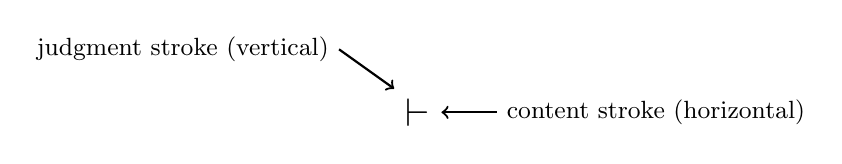
\begin{tikzpicture}
    \node at (0, 0) {\Large $\vdash$};
    \draw[<-, thick] (-0.3, 0.3) -- (-1, 0.8) node[left] {\small judgment stroke (vertical)};
    \draw[<-, thick] (0.3, 0) -- (1, 0) node[right] {\small content stroke (horizontal)};
\end{tikzpicture}
\end{center}

The \textbf{content stroke} ``---'' indicates that what follows is a proposition (something that can be true or false). The \textbf{judgment stroke} ``$|$'' asserts that this proposition \emph{has been judged true}---that we have established it.

So $\vdash \varphi$ meant: ``$\varphi$ is hereby asserted.'' Not ``$\varphi$ is true'' (a metaphysical claim), but ``$\varphi$ has been derived'' (an epistemological claim).

\begin{intuition}
Think of the judgment stroke as a \textbf{stamp of approval}. When Frege writes $\vdash \varphi$, he is saying: ``I have checked this. The derivation is complete. You may rely on $\varphi$.''

This is fundamentally a \textbf{syntactic} notion---it's about what can be written down following the rules, not about what is ``really true'' in some Platonic sense.
\end{intuition}

\subsubsection{Tarski's Turnstile: $\models$}

\begin{history}[title={Warsaw, 1933}]
Half a century later, Alfred Tarski faced a different problem: the \textbf{concept of truth itself}.

The ancient Liar Paradox (``This sentence is false'') had shown that naive talk about truth leads to contradiction. Tarski wanted a \emph{mathematically precise} definition of what it means for a sentence to be true.

His insight: truth is always \textbf{relative to an interpretation}. The sentence ``Snow is white'' is true not absolutely, but \emph{in a particular interpretation} where ``snow'' refers to snow and ``white'' means white.
\end{history}

Tarski's semantic definition of truth:
\begin{quote}
``Snow is white'' is true \emph{if and only if} snow is white.
\end{quote}

This looks circular, but it's not. The quoted sentence is a \textbf{syntactic object} (a string of symbols). The unquoted part describes the \textbf{world}. The definition connects syntax to semantics.

For formal languages, Tarski defined a \textbf{satisfaction relation}. But first: what is a \textbf{structure}?

\begin{definition}[Structure]
When a mathematician says ``a structure,'' they mean a \textbf{domain} together with \textbf{interpretations} for all the symbols in the language.

A structure $\mathcal{M}$ for a first-order language consists of:
\begin{itemize}
    \item A non-empty set $D$ called the \textbf{domain} (the ``universe'' of objects we're talking about)
    \item For each constant symbol $c$: an element $c^{\mathcal{M}} \in D$
    \item For each $n$-ary function symbol $f$: a function $f^{\mathcal{M}} : D^n \to D$
    \item For each $n$-ary relation symbol $R$: a subset $R^{\mathcal{M}} \subseteq D^n$
\end{itemize}
\end{definition}

\begin{example}[A concrete structure]
Consider the language with: constant $0$, unary function $s$ (``successor''), binary relation $<$.

One structure $\mathcal{N}$ (the natural numbers):
\begin{itemize}
    \item Domain: $D = \{0, 1, 2, 3, \ldots\}$
    \item $0^{\mathcal{N}} = 0$ (the number zero)
    \item $s^{\mathcal{N}}(n) = n + 1$ (successor adds one)
    \item $<^{\mathcal{N}} = \{(0,1), (0,2), (1,2), \ldots\}$ (the usual ordering)
\end{itemize}

A different structure $\mathcal{Z}$ using the same language:
\begin{itemize}
    \item Domain: $D = \{\ldots, -2, -1, 0, 1, 2, \ldots\}$ (all integers)
    \item $0^{\mathcal{Z}} = 0$
    \item $s^{\mathcal{Z}}(n) = n + 1$
    \item $<^{\mathcal{Z}}$ = the usual ordering on integers
\end{itemize}

Same symbols, different meanings. The sentence $\forall x\, (0 < s(x))$ is true in $\mathcal{N}$ but false in $\mathcal{Z}$ (consider $x = -1$).
\end{example}

\begin{intuition}
A structure is like a \textbf{dictionary} that tells you what each symbol \emph{refers to}. The syntax gives you sentences; the structure gives them meaning.

Different structures can make the same sentence true or false---just as ``The president is tall'' has different truth values depending on which country and time you're talking about.
\end{intuition}

Given a structure $\mathcal{M}$, we can rigorously define when $\mathcal{M}$ \emph{satisfies} a formula $\varphi$---written $\mathcal{M} \models \varphi$.

The symbol $\models$ captures this:
\begin{itemize}
    \item $\mathcal{M} \models \varphi$ means ``structure $\mathcal{M}$ satisfies $\varphi$'' (the formula is true in this interpretation)
    \item $\models \varphi$ means ``every structure satisfies $\varphi$'' (the formula is a logical truth)
    \item $\Gamma \models \varphi$ means ``every structure that satisfies all of $\Gamma$ also satisfies $\varphi$''
\end{itemize}

\begin{intuition}
Where $\vdash$ asks ``can we derive this by symbol manipulation?'', the symbol $\models$ asks ``is this true in all possible worlds?''

$\vdash$ is about \textbf{proof}. $\models$ is about \textbf{truth}.
\end{intuition}

\subsubsection{The Modern Reading}

Today, we use both symbols with refined meanings:

\begin{definition}[The syntactic turnstile $\vdash$]
$\Gamma \vdash \varphi$ means ``$\varphi$ is \textbf{derivable} from $\Gamma$ using the proof rules.''

Read as: ``$\Gamma$ \textbf{proves} $\varphi$.''
\end{definition}

\begin{definition}[The semantic turnstile $\models$]
$\Gamma \models \varphi$ means ``in every model where all of $\Gamma$ is true, $\varphi$ is also true.''

Read as: ``$\Gamma$ \textbf{entails} $\varphi$.''
\end{definition}

\begin{keyinsight}
\begin{center}
\begin{tabular}{c|c}
\textbf{Syntax} ($\vdash$) & \textbf{Semantics} ($\models$) \\
\hline
Proof, derivation & Truth, models \\
Symbol manipulation & Meaning, interpretation \\
Finite (a proof is finite) & Potentially infinite (all models) \\
\end{tabular}
\end{center}

The great theorems connect these worlds:
\begin{itemize}
    \item \textbf{Soundness}: $\vdash \varphi \Rightarrow \models \varphi$ (proofs don't lie)
    \item \textbf{Completeness}: $\models \varphi \Rightarrow \vdash \varphi$ (all truths are provable)
\end{itemize}
\end{keyinsight}

\subsection{Why Two Notions?}

Why do we need \emph{two} ways of saying ``$\varphi$ follows''?

The distinction emerged from the great foundational debates of the early 20th century:

\begin{history}[title={The Three Schools of Mathematical Philosophy}]
\textbf{Logicism} (Frege, Russell): Mathematics is reducible to logic. Mathematical truths are logical truths. This view privileges \emph{semantics}: $\models$ captures objective truth, and $\vdash$ is our attempt to systematize it.

\textbf{Formalism} (Hilbert): Mathematics is a formal game with symbols. Axioms are strings; proofs are sequences following syntactic rules. Meaning is irrelevant---what matters is consistency. This view privileges \emph{syntax}: $\vdash$ is primary, and $\models$ is a useful heuristic.

\textbf{Intuitionism} (Brouwer): Mathematics is mental construction. A statement is true only if we can \emph{construct} a proof. The law of excluded middle is rejected. Neither $\vdash$ nor $\models$ is primary---only \emph{construction} matters.
\end{history}

G\"odel's incompleteness theorems (1931) devastated the formalist program and complicated the logicist program. But the syntax-semantics distinction survived and became foundational.

\subsubsection{What Happened to the Three Schools?}

\begin{description}
    \item[Logicism] evolved into modern mathematical logic and set theory. While the original dream of reducing all mathematics to logic failed (G\"odel), the logicist spirit lives on in foundations of mathematics and type theory.

    \item[Formalism] transformed into proof theory and theoretical computer science. Hilbert's program failed in its original form, but the study of formal systems flourished. Today, automated theorem provers and proof assistants (Coq, Lean) are direct descendants.

    \item[Intuitionism] gave birth to constructive mathematics and deeply influenced computer science. The Curry-Howard correspondence---``proofs are programs''---is an intuitionist insight. Martin-L\"of type theory and dependently typed programming languages carry forward Brouwer's vision.
\end{description}

\begin{intuition}
The three schools didn't ``win'' or ``lose.'' They revealed that \emph{different questions require different foundations}:
\begin{itemize}
    \item Want to know what's true? $\models$ (semantic/logicist)
    \item Want to verify a proof mechanically? $\vdash$ (syntactic/formalist)
    \item Want to compute a witness? Construction (intuitionist)
\end{itemize}
Modern logic uses all three perspectives.
\end{intuition}

\subsection{Syntax Meets Semantics: Examples}

\begin{example}[A propositional proof]
English: ``If it rains, the ground gets wet. If the ground gets wet, the game is cancelled. It's raining. Therefore, the game is cancelled.''

Translation: Let $r$ = raining, $w$ = wet, $c$ = cancelled.
\begin{align*}
\text{Premises:} \quad & r \to w, \quad w \to c, \quad r \\
\text{Conclusion:} \quad & c
\end{align*}

\textbf{Syntactic proof}:
\begin{enumerate}
    \item $r \to w$ \hfill (premise)
    \item $w \to c$ \hfill (premise)
    \item $r$ \hfill (premise)
    \item $w$ \hfill (modus ponens: 1, 3)
    \item $c$ \hfill (modus ponens: 2, 4)
\end{enumerate}

\textbf{Semantic verification}: We check whether the formula $(r \to w) \land (w \to c) \land r \to c$ is a tautology:

\begin{center}
\begin{tabular}{ccc|ccc|c|c}
$r$ & $w$ & $c$ & $r \to w$ & $w \to c$ & \text{Premises} & $c$ & \text{Result} \\
\hline
T & T & T & T & T & T & T & T \\
T & T & F & T & F & F & F & T \\
T & F & T & F & T & F & T & T \\
T & F & F & F & T & F & F & T \\
F & T & T & T & T & F & T & T \\
F & T & F & T & F & F & F & T \\
F & F & T & T & T & F & T & T \\
F & F & F & T & T & F & F & T \\
\end{tabular}
\end{center}

\noindent where ``Premises'' = $(r \to w) \land (w \to c) \land r$. The only row where all premises are true (row 1) has $c$ = T. So Premises $\to c$ is T in all 8 rows---it's a \textbf{tautology}.

Both routes confirm validity.
\end{example}

\begin{example}[A first-order proof]
English: ``Every student respects every professor. Alice is a student. Bob is a professor. Therefore, Alice respects Bob.''

Translation:
\begin{align*}
\text{Premise 1:} \quad & \forall x \forall y \, (S(x) \land P(y) \to R(x,y)) \\
\text{Premises 2, 3:} \quad & S(a), \quad P(b) \\
\text{Conclusion:} \quad & R(a, b)
\end{align*}

\textbf{Syntactic proof}:
\begin{enumerate}
    \item $\forall x \forall y \, (S(x) \land P(y) \to R(x,y))$ \hfill (premise)
    \item $S(a)$ \hfill (premise)
    \item $P(b)$ \hfill (premise)
    \item $\forall y \, (S(a) \land P(y) \to R(a,y))$ \hfill ($\forall$-elimination on 1, $x \mapsto a$)
    \item $S(a) \land P(b) \to R(a,b)$ \hfill ($\forall$-elimination on 4, $y \mapsto b$)
    \item $S(a) \land P(b)$ \hfill ($\land$-introduction on 2, 3)
    \item $R(a,b)$ \hfill (modus ponens on 5, 6)
\end{enumerate}

\textbf{Semantic verification}: We construct a model and check that the premises entail the conclusion.

Define structure $\mathcal{M}$:
\begin{itemize}
    \item Domain: $D = \{\text{Alice}, \text{Bob}, \text{Carol}, \text{Dan}\}$
    \item Interpretation of constants: $a^{\mathcal{M}} = \text{Alice}$, $b^{\mathcal{M}} = \text{Bob}$
    \item $S^{\mathcal{M}} = \{\text{Alice}, \text{Carol}\}$ (students)
    \item $P^{\mathcal{M}} = \{\text{Bob}, \text{Dan}\}$ (professors)
    \item $R^{\mathcal{M}} = \{(\text{Alice}, \text{Bob}), (\text{Alice}, \text{Dan}), (\text{Carol}, \text{Bob}), (\text{Carol}, \text{Dan})\}$
\end{itemize}

Now verify each premise:
\begin{itemize}
    \item $\mathcal{M} \models \forall x \forall y \, (S(x) \land P(y) \to R(x,y))$? \\
    For every $d_1, d_2 \in D$: if $d_1 \in S^{\mathcal{M}}$ and $d_2 \in P^{\mathcal{M}}$, then $(d_1, d_2) \in R^{\mathcal{M}}$. \\
    Check: Alice-Bob $\checkmark$, Alice-Dan $\checkmark$, Carol-Bob $\checkmark$, Carol-Dan $\checkmark$. \textbf{True.}

    \item $\mathcal{M} \models S(a)$? Alice $\in \{$Alice, Carol$\}$. \textbf{True.}

    \item $\mathcal{M} \models P(b)$? Bob $\in \{$Bob, Dan$\}$. \textbf{True.}
\end{itemize}

Conclusion: $\mathcal{M} \models R(a,b)$? Is $(\text{Alice}, \text{Bob}) \in R^{\mathcal{M}}$? \textbf{Yes.}

The semantic route confirms: whenever all premises are true, so is the conclusion.
\end{example}
